\documentclass[10pt]{beamer}
\usetheme{SCLminimal}
\usefonttheme[onlymath]{serif}
\setbeamercovered{invisible}
\beamerdefaultoverlayspecification{<+->}

\usepackage[utf8]{inputenc}
\usepackage[english]{babel}
\usepackage[T1]{fontenc}
\usepackage{lmodern,amsmath,booktabs,setspace,mathtools,movie15}


%If you want to use section pages.
\insertsectionpages


%--------------------------------------------------------------------
%You can leave the brackets under subtitle, author and institute blank, but please retain the empty brackets.
\title[Stochastic Storm Surge Modeling \ldots]{Stochastic Storm Surge Modeling}
\subtitle{using ADCIRC+SWAN through Parallel Computing}
\singleauthor %default setting, always use on lab reports with at most 3 authors.
%\multiauthors %uncomment if true, titlepage settings for conference presentations with authors more than 3, or with multiple affiliations.
\author[VP Bo\~{n}golan, JF Rayo]{Vena Pearl Bo\~{n}golan, Ph. D.\\ Joshua Frankie Rayo}
\institute{
\sclaffiliation\\
\tref{vabongolan@dcs.upd.edu.ph, jbrayo@up.edu.ph}
   }
\event{} %presentation/conference name; default (if empty): SCL Presentation
\shortevent{}%for looong conference names; it copies the event name above if empty
\date{\today}
%--------------------------------------------------------------------





\begin{document}

{\SCLtitlepagebg
\begin{frame}[plain,noframenumbering]
  \maketitle
  \insertSCLDCSUPlogos
\end{frame}}

% TOC
\begin{frame}[noframenumbering]{Outline}
\tableofcontents
\end{frame}


\section{Introduction}
\begin{frame}{Introduction}{}
  \begin{itemize}
    \item<1-> ADCIRC is an advanced three-dimensional circulation model and a finite element numerical model for hydrodynamic circulation
    \item<1-> designed for high computational efficiency, accuracy and numerical stability
    \item<1-> provides tidal and storm related hydrodynamic forcing for simulating storm surge phenomena
    \item<2-> method: additive noise was introduced on body force
  \end{itemize}
\end{frame}

\subsection{Governing Equations}
\begin{frame}{Governing Equations}{}
  ADCIRC uses shallow water form of momentum equations coupled with continuity equation in spherical coordinates:
  \begin{block}{ADCIRC}
  	\footnotesize
  	\begin{align*}
  	\frac{\partial u}{\partial t} + u S_p \frac{\partial u}{\partial x} + v \frac{\partial u}{\partial y} + w \frac{\partial u}{\partial z} - fv &= -g S_p \frac{\partial \left[\zeta + p_s/g \rho_0 - \alpha \eta\right]}{\partial x} + \frac{\partial}{\partial z} \left(\frac{\tau_{zx}}{\rho_0}\right) - b_x + m_x \\
  	\frac{\partial v}{\partial t} + u S_p \frac{\partial v}{\partial x} + v \frac{\partial v}{\partial y} + w \frac{\partial v}{\partial z} + fu &= -g \frac{\partial \left[\zeta + p_s/g \rho_0 - \alpha \eta\right]}{\partial y} + \frac{\partial}{\partial z} \left(\frac{\tau_{zy}}{\rho_0}\right) - b_y + m_y \\
  	\nabla \cdot \vec{u} &= S_p \frac{\partial u}{\partial x} + \frac{\partial v}{\partial y} + \frac{\partial w}{\partial z} = 0
  	\end{align*}
  	\normalsize
  \end{block}
\end{frame}
%%%%%%%%%%%%%%%%

\section{Numerical Formulation}
\subsection{Variational Formulation}
\begin{frame}{Variational Formulation}{inner product wrt horizontal and vertical direction}
	\begin{figure}[H]
		\begin{center}
			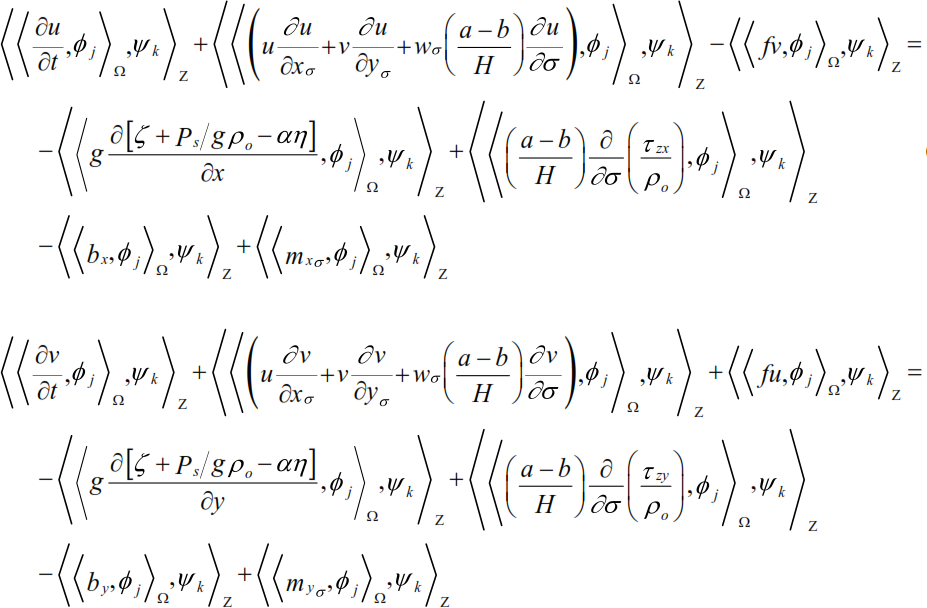
\includegraphics[width=.95\textwidth]{fem}
		\end{center}
	\end{figure}
\end{frame}

\subsection{Galerkin Finite-element Method}
\begin{frame}{Galerkin Finite-element Method}
	\begin{figure}[H]
		\begin{center}
			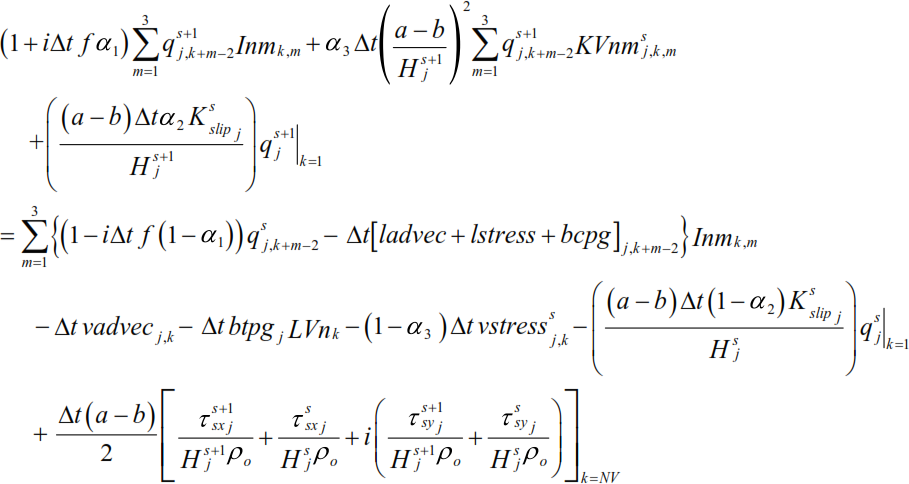
\includegraphics[width=.95\textwidth]{fem3}
		\end{center}
	\end{figure}
	Reduces to tridiagonal linear system $Mq = F$, solved by Jacobi conjugate gradient method.
\end{frame}

\section{Methodology}
\begin{frame}{Methodology}
	\begin{itemize}
		\item<1-> Noise was added to force vector $F \leftarrow F + \xi$ to simulate random external force
		\item<1-> $\xi_1 \sim \mathcal{U}(0, 10^{-4})$ and $\xi_2 \sim \mathcal{U}(0, 10^{-3})$
		\item<1-> Modified source code to include additive noise
		\item<1-> Measured elevation on three points: near Tacloban airport (1), near Tacloban main (2) and an outstanding location (3)
		\item<1-> Compared \textit{stochastic} results with \textit{deterministic} result
	\end{itemize}
\end{frame}

\begin{frame}{Methodology}{observation points}
	\begin{figure}[H]
		\begin{center}
			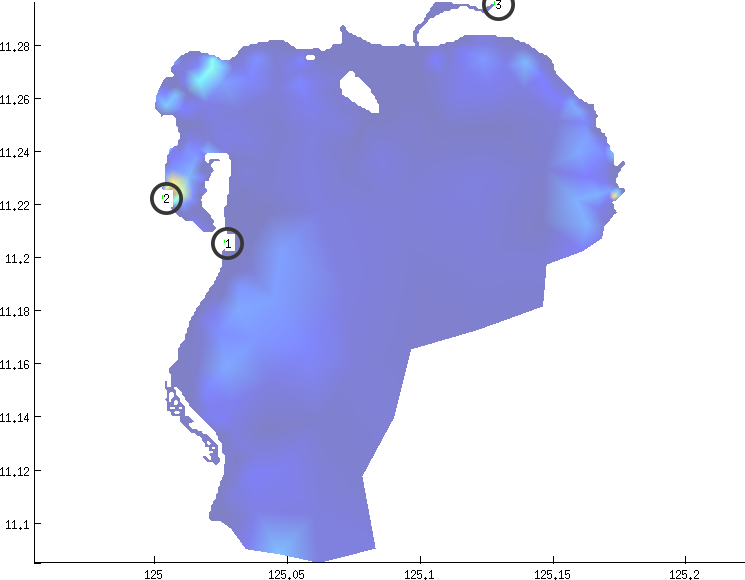
\includegraphics[width=.8\textwidth]{stations}
		\end{center}
	\end{figure}
\end{frame}

\section{Results}
\subsection{Time-series Elevation}
\begin{frame}{Time-series Elevation}{deterministic: $\xi = 0$}
	\begin{figure}[H]
		\begin{center}
			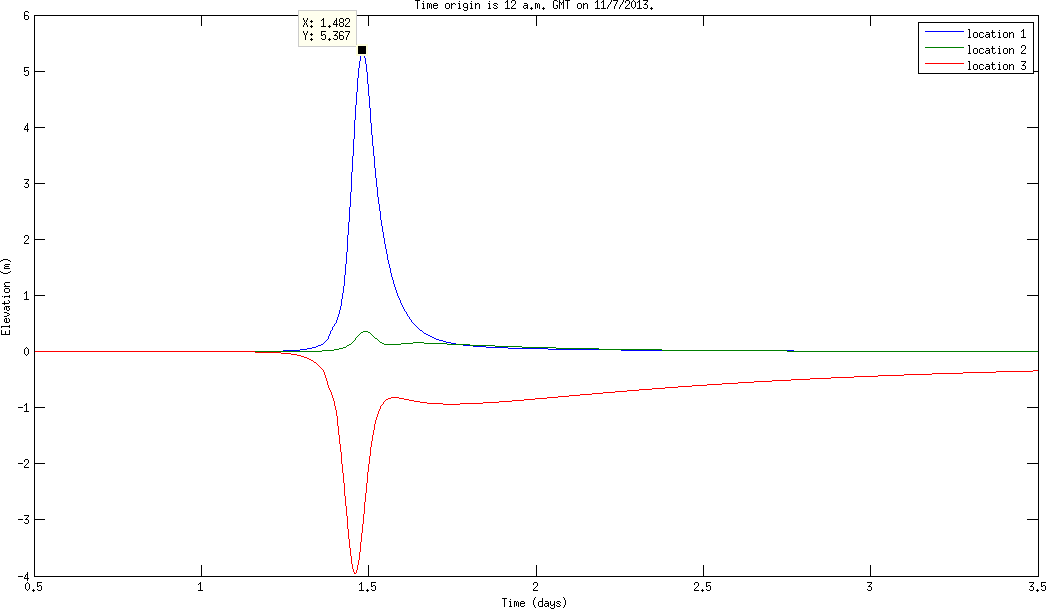
\includegraphics[width=\textwidth]{stoch0}
		\end{center}
	\end{figure}
\end{frame}

\begin{frame}{Time-series Elevation}{stochastic: $\xi_1 \sim \mathcal{U}(0, 10^{-4})$}
	\begin{figure}[H]
		\begin{center}
			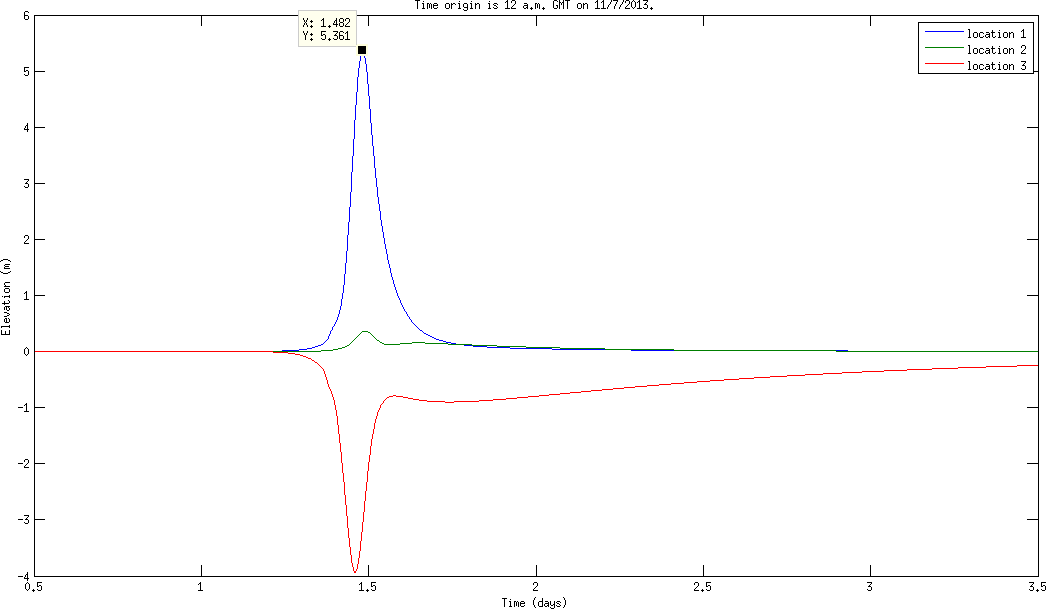
\includegraphics[width=\textwidth]{stoch2}
		\end{center}
	\end{figure}
\end{frame}

\begin{frame}{Time-series Elevation}{stochastic: $\xi_2 \sim \mathcal{U}(0, 10^{-3})$}
	\begin{figure}[H]
		\begin{center}
			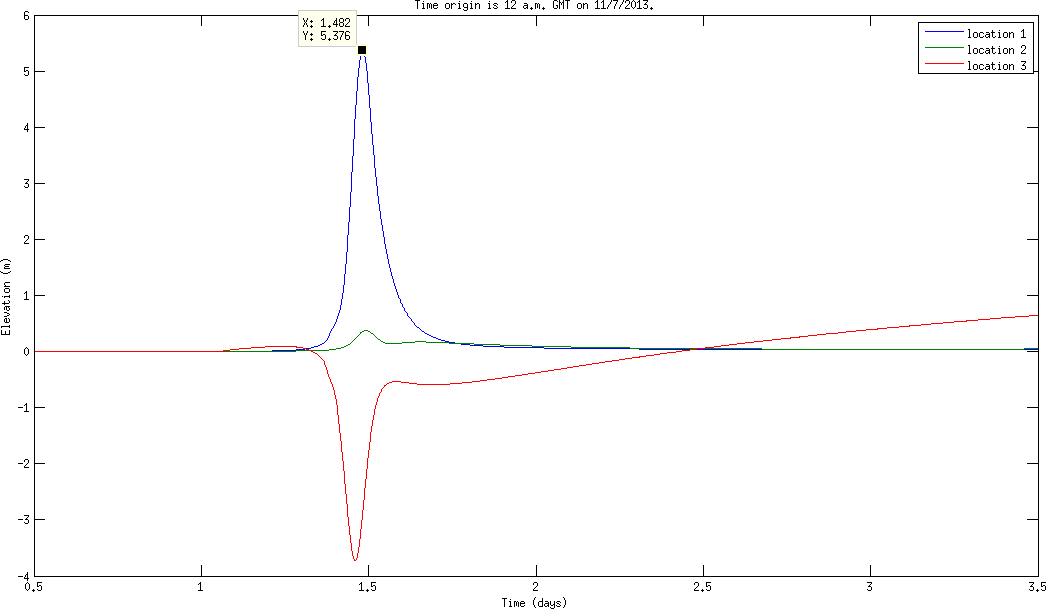
\includegraphics[width=\textwidth]{stoch1}
		\end{center}
	\end{figure}
\end{frame}

\subsection{Surge Height on Domain}
\begin{frame}{Surge Height on Domain}{deterministic: $\xi = 0$}
	\begin{figure}[H]
		\begin{center}
			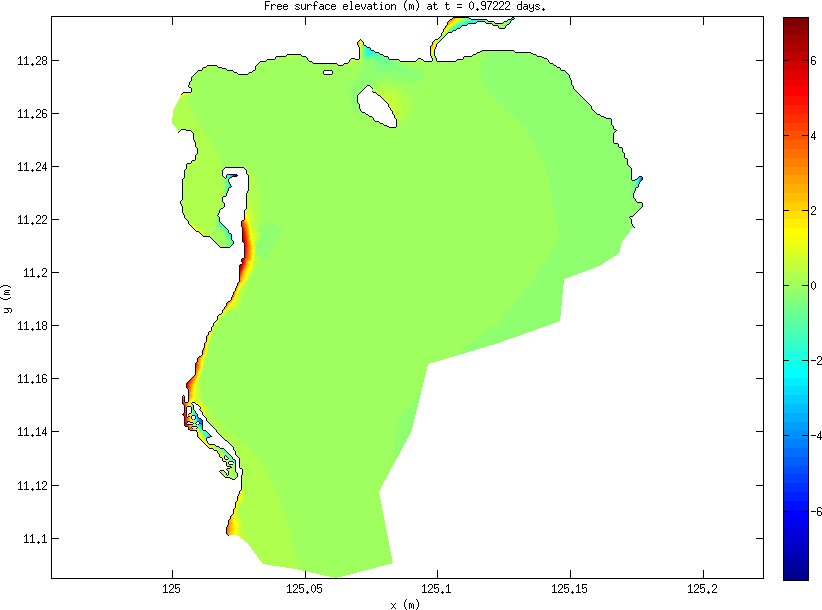
\includegraphics[width=.85\textwidth]{stoch0snap}
		\end{center}
	\end{figure}
\end{frame}

\begin{frame}{Surge Height on Domain}{stochastic: $\xi_1 \sim \mathcal{U}(0, 10^{-4})$}
	\begin{figure}[H]
		\begin{center}
			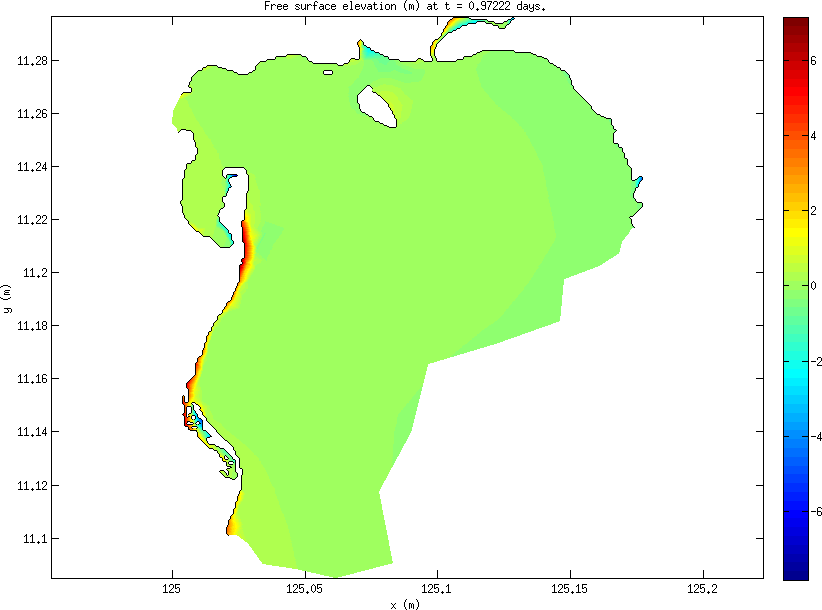
\includegraphics[width=.85\textwidth]{stoch2snap}
		\end{center}
	\end{figure}
\end{frame}

\begin{frame}{Surge Height on Domain}{stochastic: $\xi_2 \sim \mathcal{U}(0, 10^{-3})$}
	\begin{figure}[H]
		\begin{center}
			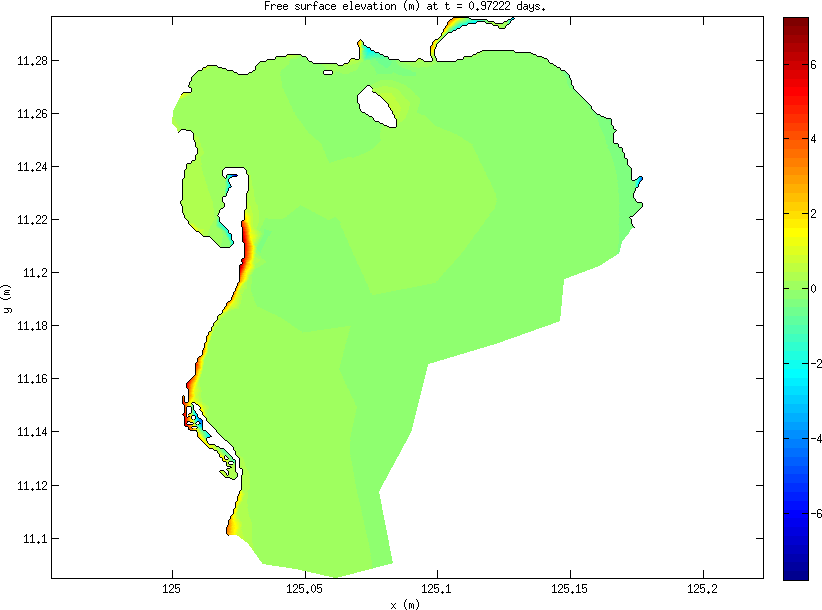
\includegraphics[width=.85\textwidth]{stoch1snap}
		\end{center}
	\end{figure}
\end{frame}


\subsection{Storm Surge Simulation}
\begin{frame}{Storm Surge Simulation}{deterministic: $\xi = 0$}
	\begin{center}
		\movie[width=.8\textwidth,height=0.6\textwidth,autostart,borderwidth=5pt,poster,autoclose,showcontrols]{}{stoch0s.avi}
	\end{center}
\end{frame}
\begin{frame}{Storm Surge Simulation}{stochastic: $\xi_1 \sim \mathcal{U}(0, 10^{-4})$}
	\begin{center}
		\movie[width=.8\textwidth,height=0.6\textwidth,autostart,borderwidth=5pt,poster,autoclose,showcontrols]{}{stoch2s.avi}
	\end{center}
\end{frame}
\begin{frame}{Storm Surge Simulation}{stochastic: $\xi_2 \sim \mathcal{U}(0, 10^{-3})$}
	\begin{center}
		\movie[width=.8\textwidth,height=0.6\textwidth,autostart,borderwidth=5pt,poster,autoclose,showcontrols]{}{stoch1s.avi}
	\end{center}
\end{frame}

\begin{frame}{Storm Surge Simulation}{side-by-side comparison}
	\begin{center}
		\movie[width=.4\textwidth,height=.3\textwidth,autostart,borderwidth=5pt,poster,repeat]{}{stoch0s.avi}
		\movie[width=.4\textwidth,height=.3\textwidth,autostart,borderwidth=5pt,poster,repeat]{}{stoch2s.avi}
		\movie[width=.4\textwidth,height=.3\textwidth,autostart,borderwidth=5pt,poster,repeat]{}{stoch1s.avi}
	\end{center}
\end{frame}

\subsection{Observations}
\begin{frame}{Observations}
	\begin{itemize}
		\item<1-> Time-series elevation curves still smooth because of the predictor-corrector algorithm employed by ADCIRC
		\item<1-> Surface elevation contours still show coherent structures despite noise
		\item<1-> Model is very sensitive to noise and larger perturbations lead to unstable computation
		\item<1-> This explains usage of uniform distribution rather than colored Levy process
	\end{itemize}
\end{frame}

\begin{frame}[noframenumbering]{Selected References}
\begin{thebibliography}{1}	
\bibitem<1->{stoch}
V. P. Bo\~{n}golan, et. al.
\newblock {\em Stochastic Terms in Boundary Conditions: Applications}.
\newblock Ellis College of the New York Institute of Technology., 2008.
	
\bibitem<1->{adcirc}
R. A. Luettich, Jr., et. al.
\newblock {\em ADCIRC: An Advanced Three-Dimensional Circulation Model, Theory and Methodology}.
\newblock US Army Engineer Waterways Experiment Station, Vicksburg, Mississippi, 1992.

\bibitem<1->{num}
R. A. Luettich, Jr., et. al.
\newblock {\em Formulation and Numerical implementation of the 2D/3D ADCIRC Finite Element Model}
\newblock \url{http://adcirc.org}, 2004.
\end{thebibliography}
\end{frame}

{\SCLendpagebg
\begin{frame}[plain,noframenumbering]
\finalpage{Thank you for your attention!}
\end{frame}}




\end{document}